
\begin{figure}[t]
\centering
\scriptsize
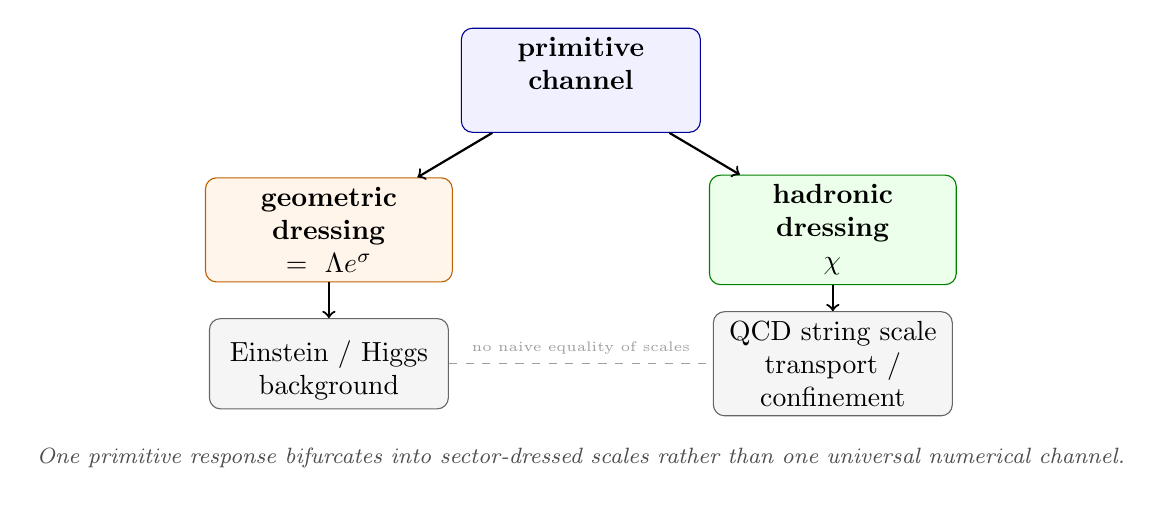
\begin{tikzpicture}[
    seed/.style={draw=blue!60!black, fill=blue!6, rounded corners, text width=2.8cm, minimum height=1.0cm, align=center},
    geo/.style={draw=orange!75!black, fill=orange!8, rounded corners, text width=2.9cm, minimum height=1.0cm, align=center},
    qcd/.style={draw=green!50!black, fill=green!8, rounded corners, text width=2.9cm, minimum height=1.0cm, align=center},
    result/.style={draw=black!60, fill=gray!8, rounded corners, text width=2.8cm, minimum height=0.95cm, align=center},
    note/.style={font=\footnotesize\itshape, text=black!70, align=center}
]
\node[seed] (seed) at (0,0) {\textbf{primitive channel}\\$\chiseed$};
\node[geo] (geo) at (-3.2,-1.9) {\textbf{geometric dressing}\\$\chigeo=\Lambda e^\sigma$};
\node[result] (geoz) at (-3.2,-3.6) {$\chigeozero$\\Einstein / Higgs background};
\node[qcd] (qcd) at (3.2,-1.9) {\textbf{hadronic dressing}\\$\chi_{\QCD}$};
\node[result] (had) at (3.2,-3.6) {QCD string scale\\transport / confinement};
\draw[->, thick] (seed) -- (geo);
\draw[->, thick] (geo) -- (geoz);
\draw[->, thick] (seed) -- (qcd);
\draw[->, thick] (qcd) -- (had);
\draw[dashed, gray!75] (geoz) -- node[above, sloped] {\tiny no naive equality of scales} (had);
\node[note] at (0,-4.8) {One primitive response bifurcates into sector-dressed scales rather than one universal numerical channel.};
\end{tikzpicture}
\caption{Local spectral-scale bifurcation. The primitive response $\chiseed$ is later dressed geometrically into $\chigeo$ and its vacuum branch $\chigeozero$, while the hadronic sector dresses the same primitive channel into $\chi_{\QCD}$. This is the clean separation that prevents the Planck/Higgs/QCD scale clash.}
\label{fig:chi-bifurcation-clean}
\end{figure}

\begin{theorem}[Geometric Hodge quantization and relative spectral gravity branch]
\label{thm:gravity-cosmology-closure}
The same geometric closure sector defines the canonical spectral gravity branch
\[
\Gamma_{\mathrm{grav}}
:=
-6\chigeo^2\mathcal E_D+\Gamma_D^{(4)}.
\]
On admissible geometric fluctuations, let
\[
Q_{\mathrm{geo}}
\]
denote the geometric BRST/Hodge differential that quotients diffeomorphism and local-frame gauge
directions, and set
\[
P_{\mathrm{phys}}^{\mathrm{grav}}
:=
\Pi_{\ker\Delta_{\mathrm{tot}}},
\qquad
\Delta_{\mathrm{tot}}
:=
\{Q_{\mathrm{adm}}+Q_{\mathrm{geo}},(Q_{\mathrm{adm}}+Q_{\mathrm{geo}})^\dagger\}.
\]
On the low-curvature local branch one recovers the effective action
\[
\begin{aligned}
\Gamma_{\mathrm{grav}}
:={}&
\int d^4x\sqrt{-g}\Big[
\frac{\Mpl^2}{2}R
-\Lambda_{\Seam,\mathrm{ren}}
+\frac{1}{6M^2}R^2
+\frac{Z_\chi}{2}(\nabla\chigeo)^2
\\
&\qquad
-U(\chigeo)
+|D\Phi|^2
-V(\Phi,\chigeo)
\\
&\qquad
-\sum_a \frac{1}{4g_a^2}\tr F_{a,\mu\nu}F_a^{\mu\nu}
+\cdots
\Big].
\end{aligned}
\]
with
\[
\Mpl^2=\frac{\chigeozero^2}{2\pi^2},
\qquad
Z_H=\frac{1}{16\pi^2},
\qquad
\vgeo^2=\frac{Z_H\mu_\Phi^2(\chigeozero)}{\lambda_\Phi}.
\]
Thus the low-curvature gravitational coefficient is later read internally as
\[
\frac{\Mpl^2}{\lambda_\Sigma^2}=\frac{\rho_\star}{2\pi^2}
\]
once the stationary boundary-normalized root has been fixed.
Its low-curvature Euler--Lagrange equations are
\[
\Mpl^2 G_{\mu\nu}
+\Lambda_{\Seam,\mathrm{ren}} g_{\mu\nu}
+\frac{1}{3M^2}\mathcal H_{\mu\nu}
=
T_{\mu\nu}^{(\chigeo,\Phi,A,\psi)},
\]
\[
Z_\chi\Box\chigeo=U'(\chigeo)+\partial_{\chigeo}V(\Phi,\chigeo),
\qquad
D^\mu D_\mu\Phi=\partial_{\Phi^\dagger}V(\Phi,\chigeo),
\]
where
\[
\mathcal H_{\mu\nu}
:=
RR_{\mu\nu}
-\frac14 g_{\mu\nu}R^2
-\nabla_\mu\nabla_\nu R
+g_{\mu\nu}\Box R.
\]
On the low-curvature vacuum branch
\[
R\ll M^2,
\qquad
\chigeo=\chigeozero,
\qquad
\Phi=\frac{1}{\sqrt2}\binom{0}{\vgeo},
\]
the theory reduces to Einstein gravity with renormalized seam vacuum energy $\Lambda_{\Seam,\mathrm{ren}}$.
On the early-universe $R^2$ branch, the Einstein-frame scalaron potential is
\[
V_{\mathrm{sc}}(\varphi)
=
\frac34 M^2\Mpl^2
\left(1-e^{-\sqrt{2/3}\,\varphi/\Mpl}\right)^2
+\Lambda_{\Seam,\mathrm{ren}}.
\]
For spatially flat FRW one has
\[
3\Mpl^2\Hhub^2
=
\frac12\dot\varphi^2+V_{\mathrm{sc}}(\varphi)+\rho_m,
\qquad
\dot{\Hhub}
=
-\frac{1}{2\Mpl^2}\bigl(\dot\varphi^2+\rho_m+p_m\bigr),
\]
and the usual slow-roll observables
\[
A_s=\frac{V_*}{24\pi^2\Mpl^4\epsilon_*},
\qquad
n_s=1-6\epsilon_*+2\eta_*,
\qquad
r=16\epsilon_*.
\]
Moreover the quadratic form of $\Gamma_{\mathrm{grav}}$ is positive on transverse traceless modes
and on the scalaron block carried by $(\chigeo,R^2)$, and null only on BRST-exact directions.
Hence the physical geometric Hilbert space takes the low-energy form
\[
\mathcal H_{\mathrm{phys}}
\cong
\mathcal H_{2}\otimes\mathcal H_{\mathrm{sc}}\otimes\mathcal H_{\mathrm{matt}},
\]
where $\mathcal H_{2}$ is the positive-helicity massless graviton sector and
$\mathcal H_{\mathrm{sc}}$ is the massive positive scalaron sector.
\end{theorem}

\begin{proof}[Proof sketch]
The canonical spectral Einstein functional of
\Cref{eq:chi-effective-action,thm:canonical-einstein-residue}, together with the local
spectral-scale formulation of \Cref{def:local-spectral-scale}, already contains the Einstein
term, the Higgs sector, the $R^2$ branch, and the gauge-curvature sector in one seam-even closure
package. The low-curvature limit freezes $\chigeo$ and $\Phi$ on the vacuum branch, while the
higher-curvature terms reduce to the retained local $R^2$ approximation used here. The same
BRST/Hodge complex kills pure geometric gauge directions cohomologically, leaving only the
transverse traceless graviton block and the positive scalaron block as physical geometric
excitations.
\end{proof}

\begin{corollary}[Classical limit]
On the vacuum branch the effective theory reproduces Einstein gravity with cosmological constant, Standard Model gauge fields, one seam-even Higgs doublet, and three chiral families.
\end{corollary}

\subsection{Absolute spectral Planck closure}

The stationary gravitational scale is no longer treated as a downstream completion block. It is read
in boundary-normalized form directly on the main theorem surface.

\begin{theorem}[Boundary spectral unit rigidity]
\label{thm:boundary-spectral-unit-rigidity}
The minimal one-sided boundary datum
\[
\Tbound=(\mathcal A_+,\mathcal H_+,D_+,J,\Gamma,B_\Sigma)
\]
determines the positive boundary spectral unit
\[
\lambda_\Sigma:=\lambda_1^+(|B_\Sigma|)=\chiseed^{-1}
\]
as a canonical, unitary-invariant spectral unit. Consequently the normalized boundary operator
\[
\widetilde B_\Sigma:=\frac{B_\Sigma}{\lambda_\Sigma}
\]
and its admissible spectral data are intrinsic invariants of the boundary branch.
\end{theorem}

\begin{proof}
The operator $B_\Sigma$ belongs to the one-sided boundary datum by
\TFPTxref{def:reduced-theorem-datum}. Hence the first positive eigenvalue of $|B_\Sigma|$ is determined
by the boundary spectrum itself. Any unitary equivalence of one-sided boundary data intertwines
$B_\Sigma$, so it preserves $\lambda_\Sigma$ and carries $\widetilde B_\Sigma$ to a unitarily
equivalent normalized operator. In particular the admissible boundary morphisms are unitary
intertwiners, not scale dilatations $B_\Sigma\mapsto c\,B_\Sigma$, so the internal spectral unit
cannot drift by a hidden rescaling.
\end{proof}

\begin{lemma}[Strict convexity in boundary units]
\label{lem:strict-convexity-rho-planck}
Define
\[
\begin{aligned}
\rho&:=\frac{\chigeo^2}{\lambda_\Sigma^2},
\\
\operatorname{Vol}_{\mathrm{vac}}&:=\operatorname{Vol}(M_{\mathrm{vac}}),
\\
\widehat V_{\mathrm{Pl}}^{\mathrm{ren}}(\rho)
&:=
\lambda_\Sigma^{-4}\operatorname{Vol}_{\mathrm{vac}}^{-1}
\Gamma_{\mathrm{TFPT}}^{\mathrm{ren}}
\bigl[\chigeo=\lambda_\Sigma\sqrt{\rho},\,g=g_{\mathrm{vac}},\,\Phi=\Phi_{\mathrm{vac}}\bigr].
\end{aligned}
\]
\[
\widehat{\mathcal E}_D:=\lambda_\Sigma^{-2}\mathcal E_D,
\qquad
\widehat U_\Sigma(\rho):=U_\Sigma(\lambda_\Sigma\sqrt{\rho}),
\]
\[
\widehat L_\Sigma(\rho):=-\log\det\nolimits_{\mathrm{adm}}(1-\widehat U_\Sigma(\rho)),
\qquad
\widehat\Gamma_D^{(4)}(\rho):=\lambda_\Sigma^{-4}\Gamma_D^{(4)}(\lambda_\Sigma\sqrt{\rho}),
\]
and
\[
\widehat{\mathcal W}(\rho):=
-6\widehat{\mathcal E}_D\rho
+\widehat\Gamma_D^{(4)}(\rho)
+\rho^2\widehat L_\Sigma(\rho).
\]
In the low-curvature shadow one has
\[
\widehat V_{\mathrm{Pl}}^{\mathrm{ren}}(\rho)=\widehat{\mathcal W}(\rho).
\]
If on the admissible geometric branch
\[
\partial_\rho^2\widehat\Gamma_D^{(4)}(\rho)>0,
\qquad
\partial_\rho^2\!\bigl[\rho^2\widehat L_\Sigma(\rho)\bigr]\ge 0
\qquad
(\rho>0),
\]
then
\[
\partial_\rho^2\widehat V_{\mathrm{Pl}}^{\mathrm{ren}}(\rho)>0
\qquad
(\rho>0).
\]
\end{lemma}

\begin{proof}
The linear term $-6\widehat{\mathcal E}_D\rho$ has vanishing second derivative, so
\[
\partial_\rho^2\widehat V_{\mathrm{Pl}}^{\mathrm{ren}}(\rho)
=
\partial_\rho^2\widehat\Gamma_D^{(4)}(\rho)
+
\partial_\rho^2\!\bigl[\rho^2\widehat L_\Sigma(\rho)\bigr].
\]
The stated positivity assumptions therefore imply strict positivity of
$\partial_\rho^2\widehat V_{\mathrm{Pl}}^{\mathrm{ren}}(\rho)$ for every $\rho>0$.
\end{proof}

\begin{theorem}[Absolute spectral Planck closure]
\label{thm:absolute-spectral-planck-closure}
\label{thm:stationary_geometric_scale_equation}
Let $\lambda_\Sigma=\lambda_1^+(|B_\Sigma|)$ and
\[
\rho:=\frac{\chigeo^2}{\lambda_\Sigma^2}.
\]
On the retained admissible geometric branch define the renormalized per-volume Planck potential by
\[
\begin{aligned}
\widehat V_{\mathrm{Pl}}^{\mathrm{ren}}(\rho)
&:=
\lambda_\Sigma^{-4}\operatorname{Vol}_{\mathrm{vac}}^{-1}
\Gamma_{\mathrm{TFPT}}^{\mathrm{ren}}
\bigl[\chigeo=\lambda_\Sigma\sqrt{\rho},\,g=g_{\mathrm{vac}},\,\Phi=\Phi_{\mathrm{vac}}\bigr].
\end{aligned}
\]
In the low-curvature shadow this reduces to
\[
\widehat V_{\mathrm{Pl}}^{\mathrm{ren}}(\rho)=\widehat{\mathcal W}(\rho)
:=
-6\widehat{\mathcal E}_D\rho
+
\widehat\Gamma_D^{(4)}(\rho)
+
\rho^2\widehat L_\Sigma(\rho).
\]
Assume
\[
\partial_\rho\widehat V_{\mathrm{Pl}}^{\mathrm{ren}}(0^+)<0,
\qquad
\partial_\rho^2\widehat V_{\mathrm{Pl}}^{\mathrm{ren}}(\rho)>0\ \text{for all }\rho>0,
\qquad
\lim_{\rho\to\infty}\partial_\rho\widehat V_{\mathrm{Pl}}^{\mathrm{ren}}(\rho)=+\infty.
\]
Then there exists exactly one positive stationary root
\[
\rho_\star>0,
\qquad
\partial_\rho\widehat V_{\mathrm{Pl}}^{\mathrm{ren}}(\rho_\star)=0.
\]
The stationary geometric scale is therefore
\[
\chigeozero=\lambda_\Sigma\sqrt{\rho_\star}.
\]
\end{theorem}

\begin{proof}
By assumption, $\partial_\rho\widehat V_{\mathrm{Pl}}^{\mathrm{ren}}$ is continuous on $(0,\infty)$
and strictly increasing there. Its value is negative near $\rho=0$ and tends to $+\infty$ for
large $\rho$. The intermediate-value theorem therefore yields at least one positive stationary root,
while strict monotonicity yields uniqueness. Since $\rho=\chigeo^2/\lambda_\Sigma^2$, the unique
stationary value is
$\chigeozero=\lambda_\Sigma\sqrt{\rho_\star}$.
\end{proof}

\begin{corollary}[Certified enclosure of the spectral Planck root]
\label{cor:computable-spectral-planck-root}
Let
\[
F_{\mathrm{Pl}}(\rho):=\partial_\rho\widehat V_{\mathrm{Pl}}^{\mathrm{ren}}(\rho).
\]
Then $F_{\mathrm{Pl}}'(\rho)>0$ for all $\rho>0$. Hence any interval
\[
[\rho_-,\rho_+]
\]
with
\[
F_{\mathrm{Pl}}(\rho_-)\le 0\le F_{\mathrm{Pl}}(\rho_+)
\]
contains exactly one root, namely $\rho_\star$. In particular the stationary Planck root admits
certified interval-arithmetic enclosures of arbitrary precision.
\end{corollary}

\begin{proof}
The derivative identity
\[
F_{\mathrm{Pl}}'(\rho)=\partial_\rho^2\widehat V_{\mathrm{Pl}}^{\mathrm{ren}}(\rho)
\]
and the strict-convexity hypothesis give $F_{\mathrm{Pl}}'(\rho)>0$. Thus $F_{\mathrm{Pl}}$ is
strictly increasing, so a sign-changing interval can contain at most one root and, by continuity, at
least one root.
\end{proof}

\begin{corollary}[Planck normalization on the stationary branch]
\label{cor:planck_normalization_stationary_branch}
On the stationary branch one has
\[
\frac{\Mpl^2}{\lambda_\Sigma^2}
=
\frac{\rho_\star}{2\pi^2},
\qquad
\frac{\Mpl}{\lambda_\Sigma}
=
\frac{\sqrt{\rho_\star}}{\sqrt2\pi},
\qquad
G_N\lambda_\Sigma^2
=
\frac{\pi}{4\rho_\star},
\]
\[
\frac{m_P}{\lambda_\Sigma}
=
\frac{2\sqrt{\rho_\star}}{\sqrt\pi},
\qquad
\lambda_\Sigma\ell_P=\lambda_\Sigma t_P
=
\frac{\sqrt\pi}{2\sqrt{\rho_\star}}.
\]
\end{corollary}

\begin{proof}
Combine
\[
\Mpl^2=\frac{\chigeozero^2}{2\pi^2}
\]
from \TFPTxref{prop:canonical-bosonic-normalization} with
\[
\chigeozero=\lambda_\Sigma\sqrt{\rho_\star}
\]
from \TFPTxref{thm:absolute-spectral-planck-closure}. The remaining identities follow from the standard
relations $\Mpl^{-2}=8\pi G_N$, $m_P=1/\sqrt{G_N}$, and $\ell_P=t_P=1/m_P$.
\end{proof}
